
\subsection{Andamento sistema del terzo ordine}
Si consideri una matrice della dinamica del seguente tipo
$$
A = \begin{pmatrix}
-3 & 3 & 0\\
-2 & 3 & 2\\
0  & -6 & -3
\end{pmatrix}
$$
lo stato iniziale del sistema è
$$
x_0 = (1 \ 1\ 1)^T
$$
Si ricavano gli autovalori e gli autovettori risolvendo il polinomio
caratteristico
$$
\left\{\begin{aligned}
\lambda &= -3 &\rightarrow& u^T=(1, 0, 1)\\
\alpha &\pm j\omega = \pm j3 &\rightarrow& u_a^T=(-1, -1 , 2),\ u_b^T = (0, -1 ,
0)
\end{aligned}\right.
$$

Si deve successivamente operare una trasformazione di coordinate
$$
Z = U_r^{-1}x = (u\ u_a \ u_b)^{-1}x
$$
la risposta libera sarà
$$
x_l = U_re^{\Lambda_r t}U_r^{-1} x_0 = U_r e^{\Lambda_r t} z_0
$$
dato che $z = U_r^{-1} x$

Si rappresenta la traiettoria dello stato nello spazio $z$

\begin{figure}[H]
 \centering
 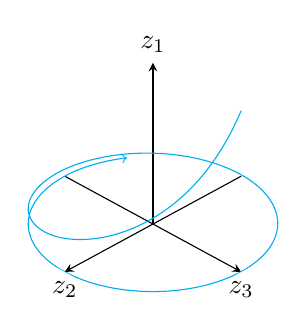
\begin{tikzpicture}
  \begin{axis}[
     axis lines = middle,
     %axis y line = center,
     view={135}{40},
     width = 0.5\linewidth,
     height =0.5\linewidth,
     xtick={0},
     ytick={0},
     ztick={0},
     xticklabels = {},
     yticklabels = {},
     zticklabels = {},
     xlabel={$z_2$},
     ylabel={$z_3$},
     zlabel={$z_1$},
     label style={at={(ticklabel* cs:1)},anchor=north},
     zlabel style={at={(ticklabel* cs:1)},anchor=south},
     ]
   \addplot3[
        color=cyan,
        domain = 0:10,
        samples = 200,
        samples y = 0,
        ->,
        ]
     ({sin(deg(x))},
     {cos(deg(x))},
     {e^(-x)});
  \end{axis}
 \end{tikzpicture}
\end{figure}

lungo l'asse $z_1$ si troverà il modo associato all'autovalore reale $\lambda$,
dunque la componente $z_1$ tenderà esponenzialmente a zero.
Le componenti $z_2$ e $z_3$ invece saranno funzioni sinusoidali ortogonali, si
otterrà un punto rotante nel piano $(z_2,z_3)$ all'estinguersi della componente
esponenziale dovuta a $z_1$.

\newpage
Per analizzare la dinamica nello spazio $x$ si deve ruotare e scalare il
sistema di riferimento $u$ rispetto a quello iniziale $x$
\begin{figure}[H]
 \centering
 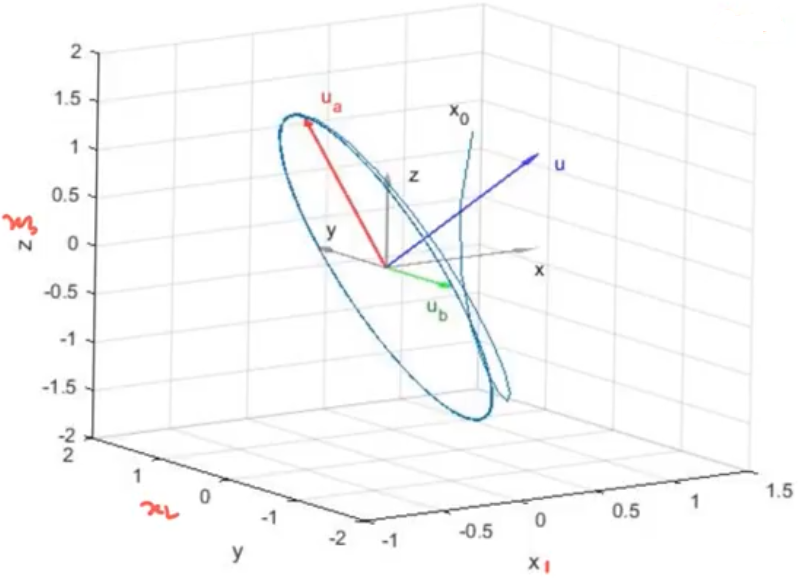
\includegraphics[width=\picwid]{traiettoria_3D_sistema_x}
\end{figure}

\subsubsection{Analisi con matrice non diagonalizzabile}
Mediante una trasformazione è comunque possibile ottenere una matrice
esponenziale diagonale a blocchi.
Nel caso di $\lambda$ reali i modi sono del tipo
$$
t^r e^{\lambda t} u
$$
con $r\in[0,\sigma-1]$ e $\sigma$ la molteplicità geometrica dell'autovalore ed
$u$ l'autovettore associato a $\lambda$.

Analisi delle componenti dello stato al variare del segno di $\lambda$ (con
$r>0$)
\begin{figure}[h]
\centering
 \begin{subfigure}[b]{0.32\textwidth}
  \centering
  \begin{tikzpicture}
   \begin{axis}[
     axis lines=left,
     %axis x line=middle,
     width=\textwidth,
     xtick={0,5},
     domain=0:5,
     xticklabels={0,t},
     ytick={0,1.5},
     xmax=5,
     ymax=1.5,
     ymin=0,
     yticklabels={0,$x_l(t)$},
     ]
    \addplot[color=red]{x*exp(-x)};
    \node[color=red] at (axis cs:0.7,0.6){$r=1$};
    \addplot[color=blue]{x^2*exp(-x)};
    \node[color=blue] at (axis cs:2.5,0.7){$r=2$};
    \addplot[color=green]{x^3*exp(-x)};
    \node[color=green] at (axis cs:4.3,1.3){$r=3$};
   \end{axis}
  \end{tikzpicture}
  \caption{$\lambda<0$}
 \end{subfigure}
\hfill
 \begin{subfigure}[b]{0.32\textwidth}
  \centering
  \begin{tikzpicture}
   \begin{axis}[
     axis lines=left,
     %axis x line=middle,
     width=\textwidth,
     xtick={0,1.2},
     domain=0:1.2,
     xticklabels={0,t},
     ytick={0},
     %xmax=3,
     %ymax=1.5,
     ymin=0,
     yticklabels={},
     ylabel={$x_l(t)$},
     ylabel style={at={(ticklabel* cs:1)},anchor=east,rotate= -90},
     ]
    \addplot[color=red]{x};
    \node[color=red] at (axis cs:0.25,0.5){$r=1$};
    \addplot[color=blue]{x^2};
    \node[color=blue] at (axis cs:0.7,0.95){$r=2$};
    \addplot[color=green]{x^3};
    \node[color=green] at (axis cs:1,0.4){$r=3$};
    \end{axis}
  \end{tikzpicture}
  \caption{$\lambda=0$}
 \end{subfigure}
\hfill
 \begin{subfigure}[b]{0.32\textwidth}
  \centering
  \begin{tikzpicture}
   \begin{axis}[
     axis lines=left,
     %axis x line=middle,
     width=\textwidth,
     xtick={0,2},
     domain=0:2,
     xticklabels={0,t},
     ytick={0},
     %xmax=3,
     %ymax=1.5,
     ymin=0,
     yticklabels={},
     ylabel={$x_l(t)$},
     ylabel style={at={(ticklabel* cs:1)},anchor=east,rotate= -90},
     ]
    \addplot[color=red]{x*exp(x)};
    %\node[color=red] at (axis cs:0.7,0.6){$r=1$};
    \addplot[color=blue]{x^2*exp(x)};
    %\node[color=blue] at (axis cs:2.5,0.7){$r=2$};
    \addplot[color=green]{x^3*exp(x)};
    %\node[color=green] at (axis cs:4.3,1.3){$r=3$};
    \end{axis}
  \end{tikzpicture}
  \caption{$\lambda>0$}
 \end{subfigure}
\end{figure}

Analizzando le tre figure
\begin{itemize}
 \item [$\lambda <0$] Il vettore di stato cresce per un certo periodo di tempo
e poi decresce fino a tendere a zero
 \item [$\lambda=0$] Il vettore cresce con andamento polinomiale
 \item [$\lambda>0$] Il vettore cresce con andamento esponenziale
\end{itemize}

\newpage
\subsubsection{Autovalori complessi e coniugati}
Si avranno due funzioni trigonometriche ortogonali tra loro moltiplicate per la
forma polinomiale $t^r e^{\alpha t}$

$$
t^re^{\alpha t} \left(\cos(\omega t +\varphi)u_a + \sin(\omega t
+\varphi)u_b\right)
$$

Si ottiene il grafico delle componenti dello stato nei tre diversi casi
\begin{figure}[h]
\centering
 \begin{subfigure}[b]{0.32\textwidth}
  \centering
  \begin{tikzpicture}
   \begin{axis}[
     axis lines=left,
     axis x line=middle,
     width=\textwidth,
     xtick={0},
     domain=0:5,
%    xticklabels={0,t},
     ytick={0},
     xmax=5,
     %ymax=1.5,
     %ymin=0,
%    yticklabels={0,$x_l(t)$},
     ylabel={$x_l(t)$},
     ylabel style={at={(ticklabel* cs:1)},anchor=east,rotate= -90},
     xlabel={$t$},
     xlabel style={at={(ticklabel* cs:1)},anchor=north},
     ]
    \addplot[color=black,samples=200]{x*exp(-x)*sin(300*x)};
    \addplot[color=red]{x*exp(-x)};
    \addplot[color=red]{-x*exp(-x)};
    \end{axis}
  \end{tikzpicture}
  \caption{$\alpha<0$}
 \end{subfigure}
\hfill
 \begin{subfigure}[b]{0.32\textwidth}
  \centering
  \begin{tikzpicture}
   \begin{axis}[
     axis lines=left,
     axis x line=middle,
     width=\textwidth,
     xtick={0},
     domain=0:5,
%    xticklabels={0,t},
     ytick={0},
     xmax=5,
     %ymax=1.5,
     %ymin=0,
%    yticklabels={0,$x_l(t)$},
     ylabel={$x_l(t)$},
     ylabel style={at={(ticklabel* cs:1)},anchor=east,rotate= -90},
     xlabel={$t$},
     xlabel style={at={(ticklabel* cs:1)},anchor=north},
     ]
    \addplot[color=black,samples=200]{x*sin(300*x)};
    \addplot[color=red]{x};
    \addplot[color=red]{-x};
    \end{axis}
  \end{tikzpicture}
  \caption{$\alpha=0$}
 \end{subfigure}
\hfill
 \begin{subfigure}[b]{0.32\textwidth}
  \centering
  \begin{tikzpicture}
   \begin{axis}[
     axis lines=left,
     axis x line=middle,
     width=\textwidth,
     xtick={0},
     domain=0:5,
%    xticklabels={0,t},
     ytick={0},
     xmax=5,
     %ymax=1.5,
     %ymin=0,
%    yticklabels={0,$x_l(t)$},
     ylabel={$x_l(t)$},
     ylabel style={at={(ticklabel* cs:1)},anchor=east,rotate= -90},
     xlabel={$t$},
     xlabel style={at={(ticklabel* cs:1)},anchor=north},
     ]
    \addplot[color=black,samples=200]{x*sin(300*x)*exp(x)};
    \addplot[color=red]{x*exp(x)};
    \addplot[color=red]{-x*exp(x)};
    \end{axis}
  \end{tikzpicture}
  \caption{$\alpha>0$}
 \end{subfigure}
\end{figure}

Sommando le due componenti si ottiene la traiettoria dello stato
\begin{figure}[h]
\centering
 \begin{subfigure}[b]{0.45\textwidth}
  \centering
  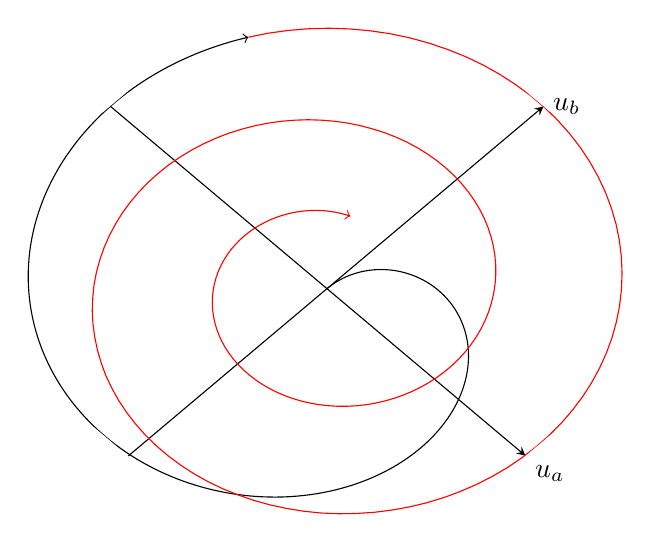
\begin{tikzpicture}
   \begin{axis}[
   view={45}{90},
     axis lines=middle,
    % axis x line=middle,
     width=\textwidth,
     xtick={0},
%    xticklabels={0,t},
     ytick={0},
     ztick={0},
     tick style={draw=none},
     z axis line style={draw=none},
     %ymax=1.5,
     %ymin=0,
%    yticklabels={0,$x_l(t)$},
     ylabel={$u_b$},
     ylabel style={at={(ticklabel* cs:1)},anchor=west},
     xlabel={$u_a$},
     xlabel style={at={(ticklabel* cs:1)},anchor=north west},
     ]
    \addplot3[
     color=black,
     samples=200,
     samples y =0,
     domain=0:1,->]
     ({x*exp(-x)*sin(300*x)},
     {x*exp(-x)*cos(300*x)},{0});
    \addplot3[
     color=red,
     samples=200,
     samples y =0,
     domain=1:3.5,->]
     ({x*exp(-x)*sin(300*x)},
     {x*exp(-x)*cos(300*x)},{0});
   \end{axis}
  \end{tikzpicture}
  \caption{$\alpha<0$}
 \end{subfigure}
\hfill
 \begin{subfigure}[b]{0.45\textwidth}
  \centering
  \begin{tikzpicture}
   \begin{axis}[
   view={45}{90},
     axis lines=middle,
    % axis x line=middle,
     width=\textwidth,
     xtick={0},
%    xticklabels={0,t},
     ytick={0},
     ztick={0},
     tick style={draw=none},
     z axis line style={draw=none},
     %ymax=1.5,
     %ymin=0,
%    yticklabels={0,$x_l(t)$},
     ylabel={$u_b$},
     ylabel style={at={(ticklabel* cs:1)},anchor= west},
     xlabel={$u_a$},
     xlabel style={at={(ticklabel* cs:1)},anchor=north west},
     ]
    \addplot3[
     color=red,
     samples=200,
     samples y =0,
     domain=0:4,->]
     ({x*exp(x)*sin(300*x)},
     {x*exp(x)*cos(300*x)},{0});
   \end{axis}
  \end{tikzpicture}
  \caption{$\alpha\geq0$}
 \end{subfigure}
\end{figure}

Gli ultimi due casi sono stati accorpati nello stesso grafico per semplicità,
in ogni caso se $\alpha$ è maggiore o uguale a zero lo stato diverge.

\newpage
\section{Analisi della risposta forzata}
L'evoluzione forzata di un sistema dipende dall'ingresso, è dunque difficile
generalizzare un'analisi senza definire a priori una serie di segnali
\textit{canonici} utilizzati con ricorrenza come segnali di ingresso per i
sistemi dinamici.

\subsection{Segnali canonici}
\label{sec:segnali_canonici}
\subsubsection{Impulso rettangolare}
Il segnale indicato con $\delta_\varepsilon(t)$ con area unitaria
\begin{figure}[h]
\centering
 \begin{tikzpicture}
  \begin{axis}
   [
    width=\picwid,
    axis lines = left,
    axis y line = middle,
    xlabel={$t$},
    ylabel={$\delta_\varepsilon(t)$},
    xmax=3,
    xmin=-1,
    ymin=0,
    ymax=1.5,
    xtick={1},
    xticklabels={$\varepsilon$},
    ytick={1},
    yticklabels={$\frac{1}{\varepsilon}$},
    xlabel style={at={(ticklabel* cs:1)},anchor=north},
   ]
   \addplot[domain=0:1,samples=2]{1};
   \draw[] (1,1)--(1,0);
  \end{axis}
 \end{tikzpicture}
\end{figure}

Descritto con la seguente
$$
\delta_\varepsilon(t) =
\begin{cases}
\frac{1}{\varepsilon} & 0\leq t <\varepsilon \\
0 & \text{altrimenti}
\end{cases}
$$
Eseguendo il limite si ottiene \textbf{l'impulso di Dirac} o \textbf{Delta di
Dirac}
$$
\lim_{\varepsilon \to 0} \delta_\varepsilon(t) = \delta(t)
$$
\textbf{Proprietà della $\delta$}
$$\left\{
\begin{aligned}
&\delta(t)=0 & \forall t\neq 0 \\
&\int_{-\infty}^{\infty} \delta(\tau)d\tau = 1\\
&f(t)\delta(t-\tau) = f(\tau)\delta(t-\tau)
\end{aligned}\right.
$$

Queste tipologie di ingressi rappresentano delle sollecitazioni
\textit{violente} al sistema, l'impulso trasferisce al sistema un'energia
finita in un tempo infinitesimo, dunque con una potenza \textit{infinita}.

È possibile rappresentare fenomeni reali con dinamiche nel tempo molto
distinte tra loro mediante la funzione impulso, ad esempio l'apertura per
pochi secondi della porta di un forno acceso da molti minuti è un fenomeno con
un tempo trascurabile rispetto all'intera dinamica del sistema ma sottrae
comunque una quantità di energia finita allo stesso; si può per questo
caratterizzare l'interazione o il forzamento mediante una funzione impulsiva.

Analogamente il colpo inferto \textit{istantaneamente} ad una biglia su un
tavolo, le conferisce istantaneamente una certa energia che la mette in moto.

\subsubsection{Segnale gradino}
Un segnale con due livelli costanti, mediante un passaggio \textit{istantaneo}
$$
\delta_{-1}(t) = \begin{cases}
0 & t<0 \\
1 & t \geq 0
\end{cases}
$$
\begin{figure}[h]
\centering
 \begin{tikzpicture}
  \begin{axis}
   [
    width=\picwid,
    axis lines = left,
    axis y line = middle,
    xlabel={$t$},
    ylabel={$\delta_{-1}(t)$},
    xmax=3,
    xmin=-1,
    ymin=0,
    ymax=1.5,
    xtick={0},
    xticklabels={0},
    ytick={1},
    yticklabels={1},
    xlabel style={at={(ticklabel* cs:1)},anchor=north},
   ]
   \addplot[domain=0:3]{1};
  \end{axis}
 \end{tikzpicture}
\end{figure}

Si può anche rappresentare con
$$
\delta_{-1}(t) = \int_{-\infty}^{t} \delta(\tau)d\tau
$$

\subsubsection{Rampa unitaria}
Indicata con
$$
\delta_{-2}(t) = \begin{cases}
0 & t<0 \\
t & t\geq 0
\end{cases}
$$
Ha il seguente andamento con pendenza unitaria
\begin{figure}[h]
\centering
 \begin{tikzpicture}
  \begin{axis}
   [
    width=\picwid,
    axis lines = left,
    axis y line = middle,
    axis equal image,
    xlabel={$t$},
    ylabel={$\delta_{-2}(t)$},
    xmax=1.5,
    xmin=-1,
    ymin=0,
    xtick={0},
    xticklabels={0},
    ytick={0},
    yticklabels={0},
    xlabel style={at={(ticklabel* cs:1)},anchor=north},
   ]
   \addplot[domain=0:1.5]{x};
  \end{axis}
 \end{tikzpicture}
\end{figure}
Analogamente al segnale precedente
$$
\delta_{-2}(t) = \int_{-\infty}^{t} \delta_{-1}(\tau)d\tau
$$

\newpage
\subsubsection{Parabola unitaria}
Un segnale che cresce con accelerazione costante
$$
\delta_{-3}(t) = \begin{cases}
0 & t<0 \\
\frac{t^2}{2} & t\geq 0
\end{cases}
$$
\begin{figure}[h]
\centering
 \begin{tikzpicture}
  \begin{axis}
   [
    width=\picwid,
    axis lines = left,
    axis y line = middle,
    axis equal image,
    xlabel={$t$},
    ylabel={$\delta_{-2}(t)$},
    xmax=1.5,
    xmin=-1,
    ymin=0,
    xtick={0},
    xticklabels={0},
    ytick={0},
    yticklabels={0},
    xlabel style={at={(ticklabel* cs:1)},anchor=north},
   ]
   \addplot[domain=0:1.5]{x^2/2};
  \end{axis}
 \end{tikzpicture}
\end{figure}
$$
\delta_{-3}(t) = \int_{-\infty}^{t} = \delta_{-2}(\tau)d\tau
$$

\subsubsection{Segnale polinomiale di ordine $n$}
Indicato con
$$
\delta_{-(n+1)}(t) = \begin{cases}
 0 & t<0 \\
 \frac{t^n}{n!} & t\geq 0
\end{cases} = \frac{t^n}{n!}\delta_{-1}(t)
$$
oppure
$$
\delta_{-(n+1)}(t) = \int_{-\infty}^{t} \delta_{-n}(\tau)d\tau
$$

\newpage
\subsubsection{Segnali comunque complessi}
I segnali polinomiali sono molto utili anche per \textit{destrutturare} segnali
più complessi, ad esempio il seguente segnale in rosso
\begin{figure}[h]
\centering
 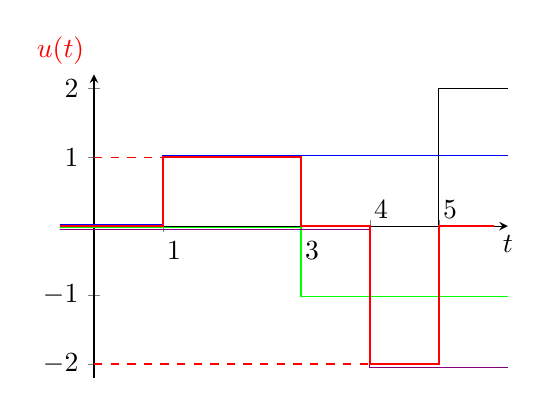
\begin{tikzpicture}
  \begin{axis}
   [
    width=0.6\linewidth,
    axis lines = middle,
    axis y line = middle,
    axis equal image,
    xlabel={$t$},
    ylabel={$u(t)$},
    xmax=6,
    xmin=-0.5,
    ymin=-2.2,
    ymax=2.2,
    xtick={1,3,4,5},
    %xticklabels={},
    ytick={-2,-1,0,1,2},
    %yticklabels={$\frac{1}{\varepsilon}$},
    xlabel style={at={(ticklabel* cs:1)},anchor=north},
    ylabel style={at={(ticklabel* cs:1)},anchor=south east,color=red},
    x tick label style={yshift={(\tick==4)*1.5em}},
    x tick label style={yshift={(\tick==5)*1.5em}},
    xticklabel style={xshift=4pt},
    ]
%   \addplot[domain=1:3,samples=2]{1};
%   \addplot[domain=4:5,samples=2]{-2};

   %\draw[] (3,0)--(3,1);
   %\draw[] ()--();
   \draw[dashed,color=red] (0,1)--(1,1);
   \draw[dashed,color=red] (0,-2)--(4,-2);
   \draw[color=blue,yshift=0.6pt] (-0.5,0)--(1,0)--(1,1)--(6,1);
   \draw[color=green, yshift=-0.6pt] (-1.5,0)--(3,0) --
   (3,-1) -- (6,-1);

   \draw[color = violet, yshift=-1.2pt] (-1.5,0)-- (4,0) --
   (4,-2)--(6,-2);
   \draw[color =black] (5,0)--(5,2)--(6,2);
   \draw[color=red,line width=0.25mm]
        (-0.5,0)--(1,0)--
        (1,1)--(3,1)--
        (3,0)--(4,0)--
        (4,-2)--(5,-2)
        --(5,0)--(5.8,0);
   \end{axis}
 \end{tikzpicture}
\end{figure}
può essere scomposto mediante una combinazione lineare di gradini
$\delta_{-1}$, sfruttando il principio di sovrapposizione degli effetti poi si
analizzerà il sistema sottoposto volta per volta a ciascuna parte del segnale
scomposto.

$$
\textcolor{red}{u(t)} = \textcolor{blue}{\delta_{-1}(t-1)}
\textcolor{green}{-\delta_{-1}(t-3) } \textcolor{violet}{- 2\delta_{-1}(t-4)} +
2\delta_{-1}(t-5)
$$
Se si volesse calcolare la risposta forzata $y_f(t)$, assumendo che $y'_f(t)$
sia la risposta al generico impulso $\delta_{-1}(t)$
$$
y_f(t) = y'_f(t-1) - y'_f(t-3) -2y'_f(t-4)+2y'_f(t-5)
$$

\newpage
\subsubsection{Segnale porta diagonale}
Sia il seguente segnale (in rosso), si vuole rappresentare la sua combinazione
lineare che lo genera
\begin{figure}[h]
\centering
 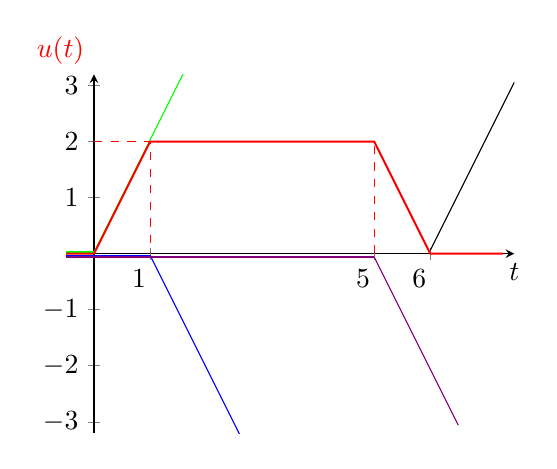
\begin{tikzpicture}
  \begin{axis}
   [
    width=0.6\linewidth,
    axis lines = middle,
    axis y line = middle,
    axis equal image,
    xlabel={$t$},
    ylabel={$u(t)$},
    xmax=7.5,
    xmin=-0.5,
    ymin=-3.2,
    ymax=3.2,
    xtick={1,5,6},
    %xticklabels={},
    ytick={-3,-2,-1,0,1,2,3},
    %yticklabels={$\frac{1}{\varepsilon}$},
    xlabel style={at={(ticklabel* cs:1)},anchor=north},
    ylabel style={at={(ticklabel* cs:1)},anchor=south east,color=red},
    %x tick label style={yshift={(\tick==4)*1.5em}},
    %x tick label style={yshift={(\tick==5)*1.5em}},
    xticklabel style={xshift=-4pt},
    ]
%   \addplot[domain=1:3,samples=2]{1};
%   \addplot[domain=4:5,samples=2]{-2};

   %\draw[] (3,0)--(3,1);
   %\draw[] ()--();
   %\draw[dashed,color=red] (0,1)--(1,1);
   %\draw[dashed,color=red] (0,-2)--(4,-2);
   %\draw[color=blue,yshift=0.6pt] (-0.5,0)--(1,0)--(1,1)--(6,1);
   %\draw[color=green, yshift=-0.6pt] (-1.5,0)--(3,0) --
   %(3,-1) -- (6,-1);

   %\draw[color = violet, yshift=-1.2pt] (-1.5,0)-- (4,0) --
   %(4,-2)--(6,-2);
   %\draw[color =black] (5,0)--(5,2)--(6,2);
   \draw[color=green, yshift=0.6pt] (-0.5,0)--(0,0);
   \addplot[domain=0:2.5,color=green,yshift=0.6pt]
           {2*x};

   \draw[color=blue, yshift=-0.6pt] (-0.5,0)--(1,0);
   \addplot[domain=1:3.5,color=blue,yshift=-0.6pt]
           {2*(1-x)};

   \draw[color=violet, yshift=-1.2pt] (-0.5,0)--(5,0);
   \addplot[domain=5:6.5,color=violet,yshift=-1.2pt]
           {2*(5-x)};

   \addplot[domain=6:7.5,yshift=1.2pt]
           {2*(x-6)};

\draw[color=red,line width=0.25mm](-0.5,0)--(0,0)--(1,2)--(5,2)--(6,0)--(7.3,0);
    \draw[color=red, dashed](0,2)--(1,2) -- (1,0);
    \draw[color=red, dashed](5,0)--(5,2);
   \end{axis}
 \end{tikzpicture}
\end{figure}
$$
\textcolor{red}{u(t)} = \textcolor{green}{+2\delta_{-2}(t)}
\textcolor{blue}{-2\delta_{-2}(t-1)}
\textcolor{violet}{-2\delta_{-2}(t-5)}
+2\delta_{-2}(t-6)
$$

\subsubsection{Rampa con gradino}
Un altro esempio
\begin{figure}[h]
\centering
 \begin{tikzpicture}
  \begin{axis}
   [
    width=0.6\linewidth,
    axis lines = middle,
    axis y line = middle,
    %axis equal image,
    xlabel={$t$},
    ylabel={$u(t)$},
    xmax=5,
    xmin=-0.5,
    ymin=-0.5,
    ymax=10,
    xtick={0,2,4},
    %xticklabels={},
    ytick={0,5},
    %yticklabels={$\frac{1}{\varepsilon}$},
    xlabel style={at={(ticklabel* cs:1)},anchor=north},
    ylabel style={at={(ticklabel* cs:1)},anchor= east,color=red},
    %x tick label style={yshift={(\tick==4)*1.5em}},
    %x tick label style={yshift={(\tick==5)*1.5em}},
    %xticklabel style={xshift=-4pt},
    ]
    \draw[color=red,line width=0.25mm]
(-0.5,0)--(0,0)--(2,5)--(4,5)--(4,0)--(4.8,0);
    \draw[color=red, dashed](0,5)--(2,5) -- (2,0);
   \end{axis}
 \end{tikzpicture}
\end{figure}

$$
u(t) = \frac{5}{2}\delta_{-2}(t) - \frac{5}{2}\delta_{-2}(t-2)-5\delta_{-1}(t-4)
$$
